\chapter{Processo de desenvolvimento da aplicação}
\label{cha:desenvolvimento}

No capítulo anterior foi apresentado o processo de desenvolvimento
e avaliação dos TCCs no curso de Ciências da Computação da UECE, como este se 
encontra atualmente. 

A partir da visão geral fornecida pelo fluxograma 
da Figura ~\ref{fig:flux_tcc} foi possível definir o comportamento básico 
da aplicação. Contudo, a aplicação não se 
detém a apenas seguir esse fluxo básico. Ela também possui funcionalidades
de alerta no sistema, para que os envolvidos no processo sejam sempre 
notificados a cada vez que um estudante, orientador ou comissão executem alguma
operação em cima de um projeto.

Neste capítulo discutiremos sobre como o sistema foi modelado, assim como sobre as
estratégias delineadas para a notificação de eventos.

\section{Escolha das tecnologias}
A seguir são apresentadas as tecnologias escolhidas como parte da plataforma de 
desenvolvimento do sistema.

\label{tecnologias}
\subsection{Linguagem de programação}
O PHP é uma linguagem de programação interpretada, multiparadigma, de código aberto, e especialmente
voltada para o desenvolvimento de aplicações para a Web. Possui uma sintaxe que lembra
C, Java e Perl, e se distingue das demais por sua facilidade de aprendizado.
Começou a ser desenvolvida em 1994 por Rasmus Lerdorf, mas o paradigma de orientação
a objetos só foi introduzido a partir da versão 3 (três), amadurecendo na versão 5 (cinco) \cite{PHP, Wiki:PHP}.

O PHP se encontra disponível na grande maioria dos servidores Web e, devido a sua 
facilidade de aprendizado, possui uma vasta comunidade de desenvolvedores. Ele é 
usado em alguns gigantes da Web, como Facebook, Wikipédia e Wordpress \cite{InfoQ:Facebook, Wikipedia:Arquitetura, Wordpress}.

Entre outros fatores, esta linguagem foi escolhida devido a sua difusão, sendo então mais
provável encontrar outros desenvolvedores que possam dar continuidade ao projeto deste trabalho,
adicionando novas funcionalidades ou corrigindo eventuais problemas.

\subsection{Framework}
De acordo com \cite{Minetto}, um framework de desenvolvimento é uma base de onde se pode desenvolver 
algo maior ou mais específico. É uma coleção de códigos-fonte, classes, funções, técnicas e 
metodologias que facilitam o desenvolvimento de novos softwares.

O uso de um framework é essencial para desenvolver uma aplicação rapidamente sem deixar
de seguir boas práticas de programação. Além disso, um programador que conheça um
framework não tem dificuldades para entender o código de outras pessoas, pois o framework obriga todos 
a seguirem as mesmas convenções. Dessa forma o programador que não conhece a aplicação pode se
manter apenas no entendimento da lógica de negócio, sem se perder na arquitetura da aplicação.

Para a aplicação desenvolvida neste trabalho, o framework escolhido foi o Symfony. O Symfony é um 
framework que possui alta aceitação na comunidade PHP, boa documentação, é patrocinado pela 
empresa francesa Sensio Labs, que garante suporte técnico a longo prazo, e tem várias outras 
qualidades que o coloca entre os melhores frameworks PHP, como:

\begin{enumerate}[a.]
\item suporte a PHP 5;
\item suporte a MVC;
\item validação de formulários;
\item extensa documentação;
\item suporte a plugins;
\item geração de código;
\item suporte a ORM e múltiplos bancos de dados;
\item convention over configuration;
\item suporte a testes unitários.
\end{enumerate}

\subsubsection{MVC}
O \sigla{MVC}{Model-View-Controller} é um acrônimo para Model-View-Controller, um padrão de projeto que tem como intuito
separar a lógica de negócio, a interface e os modelos de acesso a dados. Essa separação
de conceitos tem como propósito evitar que o código fique difícil de manter e auxilia
significamente no aumento do reuso de código. A Figura ~\ref{fig:diag_mvc} apresenta de maneira
geral a estrutura desse tipo de arquitetura.

\begin{figure}[htbp]
\centering
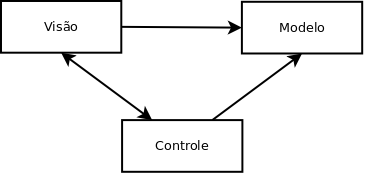
\includegraphics[width=0.5\textwidth]{fig/diagrama_mvc.png}
\caption{Arquitetura MVC}
\label{fig:diag_mvc}
\end{figure}

O modelo de acesso a dados é representado pela camada Model (ou camada de modelo). O modelo 
é um objeto que representa alguma informação sobre o domínio. É um objeto não-visual 
que contém todos os dados e comportamentos outros que não os utilizados 
pela interface \cite{Fowler:2006}.

A camada View (ou camada de visão) representa a interface da aplicação. No trabalho
em questão, ela é a parte em \sigla{HTML}{HyperText Markup Language}. Esta camada não deve possuir nenhuma lógica de negócio,
detendo-se apenas à captura e exibição de dados.

A camada Controller (ou camada de controle) é a responsável por conectar as outras duas
camadas. O controlador recebe a entrada do usuário (capturado pela visão), manipula o 
modelo e faz com que a visão seja atualizada apropriadamente \cite{Fowler:2006}.

\subsubsection{ORM}
Atualmente a maioria das aplicações é desenvolvida utilizando o paradigma de programação 
orientado a objetos apoiada por um banco de dados relacional. Essas aplicações precisam carregar
dados de um banco de dados, criar objetos para representar esses dados em memória,
executar operações em cima destes objetos e depois salvar de volta as alterações no banco.

Ferramentas de mapeamento objeto-relacional (ou \sigla{ORM}{Object-relational mapping}) são frameworks que recuperam e persistem
objetos. Seu objetivo é dar suporte à complexa atividade de gerenciar conexões entre
objetos e um banco de dados relacional. A persistência fica transparente ao desenvolvedor,
já que ele não precisa se preocupar com os detalhes de implementação. A ponte entre
objetos e seus relacionamentos é realizada pela ferramenta ORM segundo a especificação 
de mapeamento dos dados \cite{springerlink}.

\subsubsection{\emph{Convention over configuration}}
Frameworks de propósito geral normalmente necessitam de um ou mais arquivos de configuração
para serem utilizados adequadamente. Um arquivo de configuração mapeia uma classe e um recurso (uma tabela
no banco de dados) ou um evento (uma requisição web). À medida em que a complexidade das
aplicações cresce, os arquivos de configuração também crescem, tornando-se difíceis de manter \cite{Chen}. 
Para evitar este mal desnecessário, muitos frameworks atualmente procuram seguir o modelo
de desenvolvimento de software de Convenção sobre Configuração (\emph{Convention over Configuration}).
A idéia é basicamente fazer com que o desenvolvedor só precise definir aquilo que não segue 
uma convenção pré-estabelecida. 

\begin{figure}[!htbp]
\begin{minipage}[t]{0.5\linewidth}
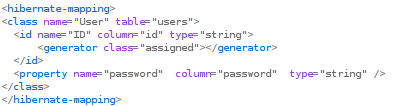
\includegraphics[scale=0.75]{fig/coc_hibernate.png}
\caption{Definição de um mapeamento no Hibernate}\label{fig:coc_hibernate}
\end{minipage} \hfill
\begin{minipage}[t]{0.3\linewidth}
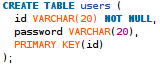
\includegraphics[scale=0.75]{fig/coc_tabela.png}
\caption{Tabela Users no banco de dados}\label{fig:coc_tabela}
\end{minipage}
\end{figure}

A Figura ~\ref{fig:coc_hibernate} apresenta um arquivo de mapeamento para Hibernate,
um framework de mapeamento objeto-relacional para Java. O código da Figura ~\ref{fig:coc_hibernate}
mapeia a classe User com a tabela Users no banco de dados. A tabela Users é descrita 
na Figura ~\ref{fig:coc_tabela} usando \sigla{SQL}{Structured Query Language}. Os campos da classe User também são mapeados
para as colunas da tabela Users.

O ato de modificar arquivos de configuração, normalmente em \sigla{XML}{eXtensible Markup Language}, é tedioso e propenso
a erros. A maioria dos problemas de configuração só vai ser detectado em tempo de execução,
disparando exceções na aplicação, que tendem a diminuir o ritmo do desenvolvimento e 
consequentemente a produtividade. Mais importante ainda, uma grande parte do
mapeamento poderia ser inferido facilmente pela estrutura da tabela sem a necessidade
de configuração alguma. Por exemplo, pode-se estabelecer uma convenção de que:
\begin{enumerate}
\item Nomes de tabelas devem ser o nome da classe no plural.
\item As colunas na tabela devem ter nomes idênticos aos campos que a classe mapeia.
\end{enumerate}

Estas duas convenções são naturais, e, de fato, já são seguidas pela maioria dos desenvolvedores.
O padrão de convenção sobre configuração reduz a quantidade de configuração ao estabelecer
um conjunto de convenções de nomenclatura que todos os desenvolvedores devem seguir \cite{Chen}.

\subsection{SGBD}
O PostgreSQL é um \sigla{SGBD}{Sistema de Gerenciamento de Banco de Dados} livre, de código aberto,
bastante robusto e confiável. Derivou-se do projeto POSTGRES da universidade de Berkley, que 
iniciou-se em 1986 e foi patrocinado por instituições militares americanas como a \sigla{DARPA}{Advanced Research Project Agency}
 (Agência de Projetos de Pesquisa Avançada para Defesa) e \sigla{ARO}{Army Research Office} (Departamento de Pesquisa Militar).
A linguagem de consultas SQL foi inserida quando o nome do projeta era Postgres95, tendo sido
rebatizado para o nome atual em 1996 para enfatizar a relação do SGBD com o SQL \cite{postgresql}.

Apesar do PostgreSQL ter sido escolhido para o desenvolvimento deste trabalho, outros SGBDs
podem ser utilizados em seu lugar, devido ao framework Symfony possuir um ORM que abstrai
a comunicação da aplicação com o banco de dados. Basta configurar a conexão do banco de dados
no Symfony e avisá-lo qual SGBD estará em uso que o seu ORM se encarregará de fazer a comunicação
correta com o banco de dados.

\subsection{IDE}
O NetBeans é um ambiente integrado de desenvolvimento (\sigla{IDE}{Integrated Development Environment}) gratuito, também de codigo aberto e 
atualmente patrocinado pela Oracle. Originalmente suportava apenas a linguagem Java, mas atualmente
consegue trabalhar com diversas linguagem de programação, entre elas o PHP, e além disso possui plugins
que facilitam a utilização de alguns frameworks, inclusive o Symfony.

Foi escolhido para este trabalho por fornecer um bom suporte ao PHP e ao Symfony, e por possuir fácil
integração com a ferramenta de depuração Xdebug, específica para PHP.

\subsection{Outros requisitos de plataforma}
Para que a aplicação funcione corretamente, é necessário que o servidor onde ela será 
atenda a alguns pré-requisitos. São eles:

\begin{itemize}
\item[PHP] Deve ser utilizada a versão 5.2.4 ou mais recente (exceto a versão 5.2.9).
\item[Servidor] Recomenda-se a utilização do servidor Apache versão 2 ou superior, com a extensão
mod\_rewrite instalada. O projeto não foi testado com outros servidores \sigla{HTTP}{Hypertext Transfer Protocol}.
\item[SGBD] Recomenda-se PostgreSQL 8.4 como SGBD por ter sido utilizado durante o desenvolvimento da aplicação, mas
de acordo com a documentação do Doctrine, o ORM do Symfony, qualquer banco de dados suportado pelo PHP através 
dos drivers PDO pode ser utilizado, já que ele utiliza \sigla{PDO}{PHP Data Objects} para se comunicar com o banco de dados.
A aplicação foi seguramente testada com MySQL Community Edition 5.5.9 e SQLite 3.7.5, podendo estes 
também serem utilizados sem prejuízo algum ao funcionamento do sistema. Para qualquer que seja o
banco escolhido, o driver PDO deve estar instalado e configurado no PHP.
\item[E-mail] É necessária uma conta de email em um servidor que aceite conexões externas via \sigla{SMTP}{Simple Mail Transfer Protocol} para
o envio das mensagens eletrônicas. Alternativamente pode-se utilizar o Sendmail, caso este esteja
configurado no servidor, ou deixar a cargo da função mail do PHP. Recomenda-se configurar um
servidor SMTP, especialmente pela facilidade de configura\-ção deste se comparado ao Sendmail. Não 
é recomendado utilizar a função mail do PHP, pois os emails enviados tendem a ser identificados
como spam em muitos servidores de email.
\end{itemize}

\section{Casos de uso e especificação de requisitos do sistema}
Para aproveitar a funcionalidade de comunicação com diferentes tipos de SGBDs, o ORM
do Symfony nos permite definir toda a estrutura do banco de dados textualmente, no formato
\sigla{YAML}{YAML Ain't Markup Language}, que possui maior legibilidade que o SQL.
A Figura ~\ref{fig:tabela_yaml} apresenta um exemplo de como as tabelas são descritas no Symfony.
Após a descrição de todas as tabelas, executamos um comando no Symfony que gera o SQL necessário
para a criação das tabelas de acordo com o SGBD escolhido. Ele também possui um comando
que gera todas as classes e formulário necessários para que possamos trabalhar com essas tabelas
que acabamos de definir.

\begin{figure}[htbp]
\centering
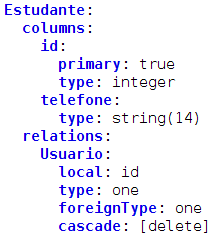
\includegraphics[width=0.25\textwidth]{fig/tabela_yaml.png}
\caption{Descrição de uma tabela no Symfony}
\label{fig:tabela_yaml}
\end{figure}

Essa geração automática de código é uma ferramenta extremamente poderosa que o framework nos
fornece para evitar perder tempo com tarefas triviais. Mas e se já tivermos começado a codificar
nas classes que ele gerou, e lembrarmos que precisamos de mais um campo na tabela? Será que
vamos ter todo o código perdido, já que ele vai sobrescrever as classes geradas automaticamente?
Isso não acontece, pois o Symfony gera duas classes para cada tabela que nós definirmos. Cada classe
herda de uma classe base abstrata, que é sobrescrita toda vez que pedimos ao Symfony que gere
as classes de acordo com a especificação. Nós temos que trabalhar em cima dessas classes que
herdam as classes bases abstratas, pois essas últimas é que o Symfony sempre vai sobrescrever.

Pra ficar mais claro, damos uma olhada no diagrama da Figura ~\ref{fig:diag_classes_base}. Ela
apresenta todas as classes base que o Symfony gerou automaticamente para a aplicação deste trabalho.
Para cada classe BaseEntidade, há uma classe Entidade, como exposto na Figura ~\ref{fig:diag_classes_principais}, 
que é criada uma única vez, caso ela ainda não exista. É nesta última que colocamos os métodos da nossa 
lógica de negócios. Tendo isso em mente, podemos prosseguir na explicação dos diagramas.

\subsection{Diagrama de classes}

A Figura ~\ref{fig:diag_classes_base} apresenta o diagrama de classes do TCC-Manager. Todas as classes
herdam direta ou indiretamente da classe sfDoctrineRecord, pertencente ao framework ORM do Symfony. 
Essa associação não foi explicitada no diagrama para que ele ficasse mais claro. A classe sfDoctrineRecord
é uma classe abstrata que possui todos os métodos de persistência dos objetos.

\begin{figure}[htbp]
\centering
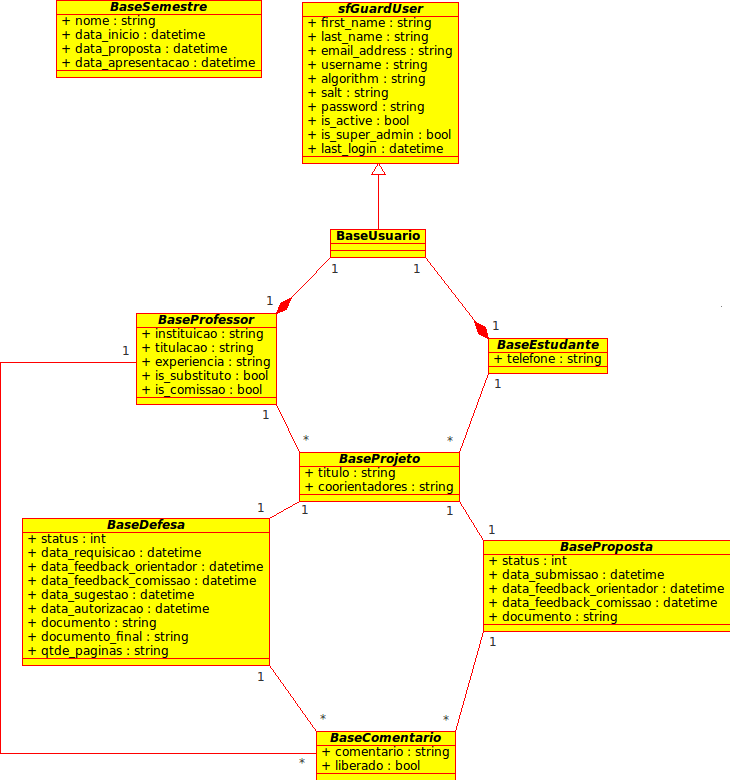
\includegraphics[width=1\textwidth]{fig/uml_classes_base.png}
\caption{Diagrama de classes base}
\label{fig:diag_classes_base}
\end{figure}

\begin{figure}[htbp]
\centering
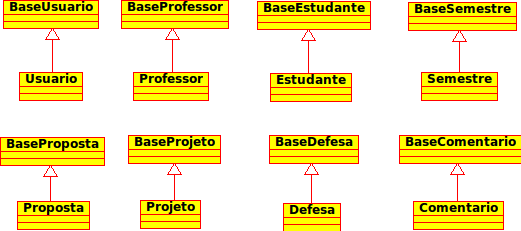
\includegraphics[width=0.7\textwidth]{fig/uml_classes_principais.png}
\caption{Diagrama de classes extendidas}
\label{fig:diag_classes_principais}
\end{figure}

A Figura ~\ref{fig:diag_classes_principais} apresenta as classes das entidades de trabalho, 
isto é, aquelas que herdam das classes base. Nelas é que deve ser inserida qualquer lógica associada
à entidade, pois o framework não escreve nessas classes, a não ser para criá-las pela primeira vez.
As classes Proposta e Defesa possuem o método audit, que é invocado quando da avaliação, por parte da comissão,
da proposta ou da solicitação de defesa. Cada vez que um professor integrante da comissão dá seu parecer,
este método salva as informações do integrante, seu parecer e um possível comentário feito por ele
sobre a proposta/defesa. Além disso, ele calcula o parecer final dependendo da decisão da maioria 
da comissão. Essas duas entidades também guardam uma enumeração que indica seu status, que podem ser os
seguintes:

\begin{itemize}
\item NAO\_ANALISADO: Proposta/Defesa não analisada
\item APROVADO: Proposta/Defesa aprovada pelo orientador
\item REPROVADO: Proposta/Defesa reprovada pelo orientador
\item LIBERADO: Proposta/Defesa aprovada pela comissão
\item NAO\_LIBERADO: Proposta/Defesa reprovada pela comissão
\end{itemize}

A classe Projeto possui alguns métodos de verificação de situação. Os nomes dos métodos são bem 
autodescritivos e indicam se o projeto possui uma proposta/defesa, se o estudante anexou o documento
da proposta ou a cópia da monografia na solicitação de defesa, e se o projeto já pode ser defendido.

\begin{figure}[htbp]
\centering
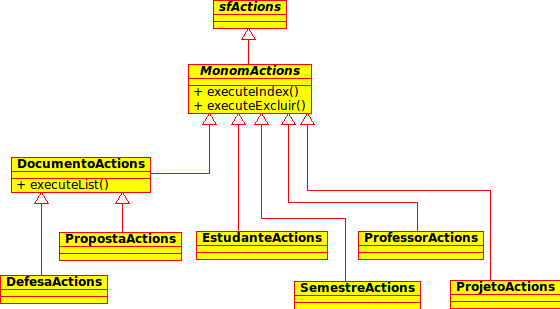
\includegraphics[width=0.7\textwidth]{fig/uml_controllers.png}
\caption{Diagrama de classes da camada de controle}
\label{fig:diag_controllers}
\end{figure}

A Figura ~\ref{fig:diag_controllers} apresenta o diagrama de classes para a camada de controle.
A classe sfActions pertence ao Symfony e cuida da comunicação entre o navegador e a aplicação. 
Internamente é ela que instancia as classes necessárias para a execução do framework; decodifica
a \sigla{URL}{Uniform Resource Locator} da requisição, de forma a determinar qual ação e qual módulo estão 
sendo requisitados, e se não existirem, exibe uma mensagem de página não encontrada; recebe os
parâmetros de entrada; chama a ação do módulo requisitado e renderiza a saída. 

Na classe de controle monomActions encontram-se métodos de \sigla{CRUD}{Create, Retrieve, Update e Delete} 
padronizados, e que são usados pela maior parte dos módulos da aplicação. A classe de controle
documentoActions contém métodos de controle de upload de arquivos, que são usados nos módulos de 
proposta e defesa. Dessa forma, foi possível fazer um grande reuso de código.


\subsubsection{Autenticação de usuários}
Na Figura ~\ref{fig:diag_classes_base} podemos observar a classe sfGuardUser, da qual a classe Usuario extende.
Ela vem de um plugin para o Symfony de controle de usuários, que oferece recursos de segurança
e autorização em cima dos recursos de segurança oferecidos pelo framework. Aproveitamos esse plugin
para fazer um bom reuso de código e contar com toda a segurança que o plugin já disponibiliza \cite{sfguardplugin}.

As classes Estudante e Professor possuem um relacionamento de composição com a classe Usuario.
Inicialmente foi pensado em fazer com que essas classes herdassem da classe Usuario, mas visto
que existe o usuário administrador que não é nem estudante, nem professor, a modelagem não pôde
ser feita dessa forma. De qualquer forma, só podem existir estudantes e professores se houver um usuário
associado a eles.

Na classe Usuario encontram-se os dados mais básicos de cada usuário, como nome, endereço de email e senha.
Há ainda outras informações que dizem respeito a como a senha é criptografada no banco de dados. 
O campo algorithm contém o algoritmo utilizado para criptografar a senha, que por padrão é o SHA1. 
Outros algoritmos podem ser utilizados, como o MD5, mas optou-se por deixar o algoritmo padrão.
O campo salt é uma string que é concatenada à senha antes da criptografia, para dificultar a a 
descoberta do valor original.

\subsubsection{Formulários}
Além de gerar as entidades, o Symfony também possui a funcionalidade de gerar formulários que
possuem validação própria. Dessa forma, só é necessário ajustar detalhes de aparência ou
validações mais complexas, como datas que devem preceder umas às outras ou valores que devem 
estar dentro de um conjunto fechado.

\begin{figure}[htbp]
\centering
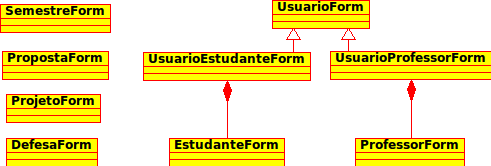
\includegraphics[width=0.5\textwidth]{fig/uml_forms.png}
\caption{Diagrama de classes dos formulários}
\label{fig:diag_forms}
\end{figure}

A Figura ~\ref{fig:diag_forms} apresenta os formulários que foram gerados a partir da descrição 
do esquema do banco de dados. Todas as classes desse diagrama herdam das suas correspondentes 
classes base, assim como acontece com as classes da Figura ~\ref{fig:diag_classes_principais}.
Elas não são apresentadas aqui por efeito de clareza no diagrama. As classes base, por sua vez,
herdam da classe BaseFormDoctrine, do framework, que possui os métodos básicos de validação e 
persistência dos formulários. 

O formulário do Anexo ~\ref{anx:proposta} é representado no sistema pelos formulários de estudante, 
professor, projeto e proposta. O formulário do Anexo ~\ref{anx:defesa} é representado no sistema 
pelos formulários de estudante, professor, projeto e defesa. 

\subsubsection{Casos de uso}
Para a execução deste projeto, foram escritos os casos de uso de uma forma básica, de maneira a não
tomar muito tempo que seria usado na codificação. Os casos de uso encontram-se listados no Apêndice ~\ref{app:casos_de_uso}.
